\documentclass[conference,a4paper]{IEEEtran}

\IEEEoverridecommandlockouts

\usepackage{cite}

\usepackage{amsmath,amssymb,amsfonts}

\usepackage{algorithmic}

\usepackage{graphicx}

\usepackage{textcomp}

\usepackage{enumitem}

\usepackage{booktabs}

\usepackage{url}

\def\IEEEkeywordsname{Keywords}

\def\BibTeX{{\rm B\kern-.05em{\sc i\kern-.025em b}\kern-.08em

\kern-.1667em\lower.7ex\hbox{\rm X}}}

\begin{document}

\title{Single-Pass Uncertainty Heads for Claim-Level Hallucination Detection in Persian Medical Language Models}

\author{\IEEEauthorblockN{Mehrdad Ghassabi}

\IEEEauthorblockA{\textit{Faculty of Computer Engineering} \\
\textit{University of Isfahan} \\
Isfahan, Iran \\
m.ghassabi@eng.ui.ac.ir}

\and

\IEEEauthorblockN{Pedram Rostami}

\IEEEauthorblockA{\textit{School of Electrical and Computer Engineering} \\
\textit{University of Tehran} \\
Tehran, Iran \\
pedram.rostami@ut.ac.ir}

\and

\IEEEauthorblockN{Hamidreza Baradaran Kashani}

\IEEEauthorblockA{\textit{Faculty of Computer Engineering} \\
\textit{University of Isfahan} \\
Isfahan, Iran \\
hrb.kashani@eng.ui.ac.ir}

\and

\IEEEauthorblockN{Sadra Hakim}

\IEEEauthorblockA{\textit{School of Computer Science} \\
\textit{University of Windsor} \\
Windsor, Canada \\
hakim6@uwindsor.ca}

\and

\IEEEauthorblockN{Audrina Ebrahimi}

\IEEEauthorblockA{\textit{Center for Brain Health} \\
\textit{University of Texas at Dallas} \\
Dallas, TX, USA \\
audrina.ebrahimi@utdallas.edu}

}

\maketitle

\begin{abstract}
Hallucination detection is important for medical language models because fluent answers can contain unsupported claims. Repeated-sampling methods estimate uncertainty by generating several answers to the same question and comparing them, but this requires multiple completions. We adapt the LLM Uncertainty Head (LUH) framework to Persian medical language models derived from Aya-Expanse-8B and construct two paired, claim-level uncertainty datasets in Persian. Each dataset contains 1,600 responses generated by Gaokerena-V or Gaokerena-R. The selected question inventory is disease-heavy: 80.6\% of entities come from the disease list and 19.4\% from a combined anatomy, laboratory-test, and procedure block; specialty-level labels are unavailable. The heads use internal attention and token-probability signals associated with one response to estimate claim-level hallucination risk. Two medical experts independently reviewed a 200-claim sample and could consult medical sources; their three-way agreement was 91.5\% (Cohen's $\kappa=0.855$). On the held-out response splits, the heads achieve PR-AUCs of 0.4820 and 0.4652 and ROC-AUCs of 0.7852 and 0.7810, respectively. We also measure five-run answer variability for Aya-Expanse-8B and its two evaluated Persian medical derivatives on a 168-question medical examination. The observed differences caution against assuming that medical adaptation or shared model lineage guarantees response consistency.
\end{abstract}

\begin{IEEEkeywords}

Small Language Models, Uncertainty Quantification, Hallucination Detection, Low-Resource Language, Persian Language Models

\end{IEEEkeywords}

\section{Introduction}
Large language models (LLMs) are increasingly used in settings where unreliable outputs can have serious consequences. In medical question answering, a generated answer may mix correct statements with unsupported claims; identifying individual claims that require verification is therefore useful even when the generator itself is not modified. This problem is particularly relevant for Persian, for which medical evaluation resources and language-specific tools remain limited.

A common approach to uncertainty estimation is to generate several answers to the same question and measure their agreement. Consistency-based methods can be informative, but they require repeated generation and usually provide a response-level signal. White-box models offer another approach: internal signals, such as attention patterns and token probabilities, can be used by an auxiliary head to estimate uncertainty for claims in a single generated response. In this paper, \emph{single-pass} refers to this single-response setting: the detector estimates uncertainty from internal signals associated with one answer instead of generating multiple answers and comparing them. It does not mean that feature extraction and auxiliary scoring are computationally free, nor does it imply that no additional forward computation is used to recover features from a stored response.

We adapt the LLM Uncertainty Head (LUH) framework of Shelmanov et al.~\cite{b1} to the Aya-Expanse-8B backbone and two Persian medical models derived from it, Gaokerena-V and Gaokerena-R~\cite{b2,b3}. LUH uses a lightweight trainable head over model-internal features while keeping the language-model backbone frozen. Because the head depends on backbone features and tokenization, adapting it to a different model family and language requires Persian claim labels and token alignment suitable for the target backbone.

This study has three objectives: (1) adapt LUH to Persian medical language models; (2) collect claim-level uncertainty data for Persian medical usage; and (3) examine response variability in Aya-Expanse-8B and its evaluated Persian medical derivatives. The third objective is an empirical caution: the consistency of a base model should not be assumed to carry over unchanged to models derived from it, and medical adaptation should not be treated as a guarantee of answer reliability. Our evidence is limited to the three 8B models and one examination task evaluated here.

The contributions are:
\begin{enumerate}[leftmargin=*]
\item \textbf{Adapting LUH to Persian models:} We adapt the LUH framework to Aya-Expanse-derived Persian medical models, training new uncertainty heads over backbone-internal attention and token-probability signals.
\item \textbf{Collecting Persian medical uncertainty data:} We construct two paired claim-level datasets, each containing 1,600 Persian medical responses, extracted claims, veracity labels, and token-level supervision. A sample of the automatic labels is independently reviewed by two medical experts with access to medical sources.
\item \textbf{An empirical caution about model-family uncertainty:} We measure five-run answer variability for Aya-Expanse-8B, Gaokerena-V, and Gaokerena-R on an Iranian medical examination. The results show that the tested base and derived models differ in response consistency, cautioning against inferring reliability from model lineage or medical fine-tuning alone.
\end{enumerate}
\section{Background and Related Work}
\subsection{Uncertainty and Hallucination Detection}
Uncertainty-estimation methods for LLMs include verbal confidence, internal-signal methods, consistency across sampled generations, and semantic clustering~\cite{b4}. Internal-signal methods use information already represented by a white-box model, whereas consistency methods compare multiple completions. In medical applications, uncertainty estimates can help identify claims requiring additional verification rather than replace it~\cite{b5,b6}. Recent work also trains auxiliary heads for claim- or reasoning-step verification while keeping the generator fixed~\cite{b7}.

\subsection{Aya-Expanse and Gaokerena}
Aya-Expanse is a multilingual family designed to improve performance across languages, including underrepresented ones~\cite{b8,b9,b10}. Gaokerena-V and Gaokerena-R are Persian medical models derived from Aya-Expanse-8B~\cite{b2,b3}; the former is medically adapted and the latter is reasoning-oriented. We use them as fixed backbones and do not claim their original model development as a contribution here.

\subsection{LLM Uncertainty Heads}
LUH trains a lightweight auxiliary Transformer head over internal features, including attention and token-probability signals, while freezing the language-model backbone~\cite{b1}. Because these features and tokenization are backbone-specific, the released heads cannot be assumed to transfer unchanged to Aya-Expanse-derived models. Similarly, translating an English claim dataset would require Persian claim-span extraction and token realignment. We therefore train new heads using claims and labels collected directly from Persian responses.

\section{Response Variability}

Before training the uncertainty heads, we examine whether repeated generations exhibit measurable variability. We evaluate Aya-Expanse-8B, Gaokerena-V, Gaokerena-R, and Med-Gemma~\cite{b11} on the September 2023 Iranian Basic Medical Sciences Entrance Examination (IBMSEE), containing 168 questions. Each model is run five times on the same questions using chain-of-thought prompting~\cite{b12}.

\subsection{Metrics}
For each question, we extract the final option letter (A--D) from each run. Invalid outputs (19/840 for Gaokerena-V, 35/840 for Gaokerena-R, and 19/840 for Aya-Expanse) are excluded from the option distribution and counted as incorrect for ensemble accuracy. Ensemble accuracy uses the option receiving at least three of five votes; questions without a majority are incorrect. We also report the number of questions with the same valid option in all five runs and the number in which all four options occur. For question $q$, let $p_{q,o}$ be the fraction of valid runs selecting option $o$. Mean per-question entropy is
\begin{equation}
H_q=-\sum_{o\in\{A,B,C,D\}}p_{q,o}\log_2 p_{q,o},
\end{equation}
where $0\log_2 0=0$; invalid runs are excluded and a question with no valid run is assigned zero entropy. With five runs and four options, the maximum is approximately 1.92 bits. Figure~\ref{fig:response_variability} visualizes both entropy and exact five-run agreement.

\begin{table}[ht]

\centering

\small

\caption{Five-run consistency on the September 2023 IBMSEE. Accuracy is the ensemble-answer accuracy (\%) with not-agreed questions counted as incorrect; entropy is the mean per-question Shannon entropy in bits over valid runs (see text).}

\label{tab:instability}

\resizebox{\columnwidth}{!}{%

\begin{tabular}{|l|c|c|c|c|}

\hline

& \textbf{Gao} & \textbf{Gao} & \textbf{Aya-} & \textbf{Med-} \\

& \textbf{kerena-V} & \textbf{kerena-R} & \textbf{Expanse} & \textbf{Gemma} \\ \hline

Accuracy & 29.76 & 38.69 & 35.71 & 37.50 \\ \hline

Questions with a & 14 & 37 & 36 & 168 \\

single option taken &  &  &  &  \\ \hline

Questions with all  & 10 & 4 & 6 & 0 \\

 options taken &  &  &  & \\ \hline

Entropy (bits) & 1.11 & 0.80 & 0.84 & 0 \\ \hline

Prompt & CoT & CoT & CoT & CoT \\ \hline

Parameters & 8B & 8B & 8B & 4B \\ \hline

\end{tabular}}

\end{table}

\begin{figure*}[!t]
\centering
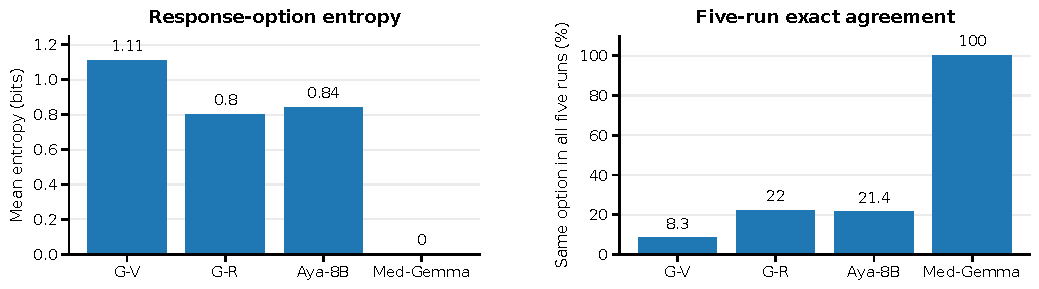
\includegraphics[width=\textwidth]{figures/fig1_response_variability.pdf}
\caption{Five-run response variability on the 168-question September 2023 Iranian Basic Medical Sciences Entrance Examination. Entropy is computed over valid answer options; exact agreement is the percentage of questions for which all five valid runs select the same option. Med-Gemma is a 4B comparison model, not an Aya-Expanse derivative.}
\label{fig:response_variability}
\end{figure*}




\subsection{Findings}

Med-Gemma returned the same option in all five runs for all 168 questions, compared with 14 questions for Gaokerena-V, 37 for Gaokerena-R, and 36 for Aya-Expanse-8B. Gaokerena-V also had the highest entropy (1.11 bits) and lowest ensemble accuracy (29.76\%); no option reached a three-vote majority on 48 questions for Gaokerena-V, 32 for Gaokerena-R, and 28 for Aya-Expanse-8B. Gaokerena-R was close to Aya-Expanse-8B in consistency and entropy and had the highest ensemble accuracy among the three 8B models. Only 4--10 questions per model contained all four options, so this row is not interpreted further. These results show differing consistency profiles among the tested base and derived models, not a general ranking of the Aya-Expanse family. The experiment motivates claim-level scoring from one response, while recognizing that internal-feature extraction and auxiliary scoring also incur overhead.

\section{Native Persian Claim-Level Dataset}

Transferring LUH to Persian requires supervision aligned with both Persian responses and the target tokenizer. Rather than translating an English dataset and then re-establishing claim and token alignment, we construct the datasets directly in Persian. The same questions are answered by both backbones, allowing the resulting datasets to be paired.

\subsection{Dataset Construction}

The pipeline has five stages. First, we select 1,600 Persian medical questions from an ordered entity pool, keeping at most one question per base entity and limiting synthetic variants to about 6\%. Second, Gaokerena-V and Gaokerena-R answer the same questions in the same order using greedy decoding, creating paired datasets at the question level. Third, Persian prompting extracts atomic, verifiable claims from each response; sentences shorter than 40 characters after markup removal are treated as headings or labels and excluded. Fourth, DeepSeek-V4-Flash~\cite{b13} labels each claim as supported, hallucinated, or undecided. Undecided claims remain in the released data but are excluded from the supervised loss; a medical-expert review of a sample is reported in Section~\ref{sec:annval}. Fifth, supported and hallucinated claims are aligned to Aya-Expanse token spans: tokens inside a claim receive its binary label and tokens outside supervised claims are masked with $-100$. The alignment procedure and its limitations are detailed in Section~\ref{sec:align}.

Table~\ref{tab:data} summarizes the resulting paired datasets. The table reports not only the number of responses and extracted claims, but also the supported and hallucinated counts, undecided claims, hallucination rates, supervised-token coverage, and the positive-class weights used during training. These statistics make two properties of the resource explicit: the two backbones contribute similar hallucination prevalences despite producing different response lengths and claim counts, and the class imbalance is substantial enough to require weighted supervision.

\begin{table}[ht]

\centering

\small

\caption{Statistics of the two native Persian uncertainty datasets.}

\label{tab:data}

\resizebox{\columnwidth}{!}{%

\begin{tabular}{|l|c|c|}

\hline

& \textbf{LUH-V} & \textbf{LUH-R} \\ \hline

Annotated responses & 1,600 & 1,600 \\ \hline

Extracted claims & 60,434 & 54,209 \\ \hline

Supported claims & 48,991 & 43,305 \\ \hline

Hallucinated claims & 10,557 & 9,528 \\ \hline

Undecided claims & 886 & 1,376 \\ \hline

Hallucination rate & 17.73\% & 18.03\% \\ \hline

Claims per response (mean) & 37.8 & 33.9 \\ \hline

Supervised tokens (\% of all input tokens) & 61.4\% & 54.9\% \\ \hline

Positive class weight & 4.64 & 4.53 \\ \hline

\end{tabular}}

\end{table}

Table~\ref{tab:data} shows 60,434 and 54,209 aligned claims, with similar hallucination rates (17.73\% and 18.03\%). Differences in undecided counts and supervised-token coverage reflect backbone-specific responses and claim spans. Claim counts include only claims with non-empty aligned spans; supervised-token coverage is calculated over all input tokens, with prompt tokens masked.

Each dataset is divided into training, validation, and test splits containing 1,458, 92, and 50 responses, respectively. The splits are sampled at even intervals across the ordered entity pool rather than taking contiguous blocks, so all three partitions cover the topical range. With only 50 test responses, the test split cannot cover every initial letter; its entities start with 16 of the 30 Persian initial letters that occur in the selection (22 for the evaluation split, all 30 for the training split), and its share of entities from the first block of the entity list (20\%) matches that of the full selection (19\%); see Section~\ref{sec:stats}.

\subsection{Pairing of the Two Datasets}
\label{sec:pairing}
Both datasets contain the same 1,600 questions in the same order and use identical train/validation/test assignments; hence, their 50 test questions are also identical. The responses, sentences, claims, token sequences, and labels are backbone-specific: no answer is identical across the datasets, and claims are not matched across backbones. Pairing therefore controls the questions, not the answers. The per-question hallucination rates are positively correlated (Spearman $\rho=0.38$, versus approximately 0.00 after random re-pairing), and paired answers share more vocabulary (mean word-set Jaccard overlap 0.32 versus 0.18 for answers to different questions). This supports using paired questions when comparing the two heads.

\subsection{Dataset Composition and Label Distribution}
\label{sec:stats}
The 3,200-question candidate inventory uses a single Persian template (``Tell me everything you know about X''), so wording is fixed and the entity varies. The selected 1,600 questions cover 1,600 base entities: 1,504 real entities and 96 synthetic ``type~$N$'' variants (6.0\%). The inventory comprises a first block of anatomical structures, laboratory tests, and procedures, plus an alphabetically ordered disease list; the selected questions include 310 (19.4\%) and 1,290 (80.6\%) from these blocks, respectively. No medical-specialty labels are available, so we do not claim specialty-balanced coverage. % AUTHOR CHECK: Add the candidate inventory source, Persian translation procedure, and provenance of the first block and synthetic variants before submission.

\subsection{Topic Coverage and Representativeness}
The documented inventory supports a two-block quantitative analysis, rather than a fine-grained specialty breakdown. The combined block of anatomical structures, laboratory tests, and procedures accounts for 310 of the 1,600 selected entities (19.4\%); the disease list accounts for the remaining 1,290 (80.6\%). Thus, the selected inventory is weighted toward disease entities. The first block nevertheless spans several biomedical areas in the released examples: basophils and blood-related tests (including ferritin, hematocrit, platelet count, and prothrombin time); hepatobiliary and digestive anatomy (bile duct and duodenum); respiratory anatomy (bronchioles and epiglottis); neuroanatomy (cerebellum and dendrites); ocular structures (choroid and cornea); and reproductive anatomy (endometrium). These are illustrative examples visible in the dataset viewers, not a complete, independently coded distribution of all entities.

The disease entries add breadth across disease concepts, but the released inventory does not provide specialty, organ-system, or ontology labels for each disease. We therefore report the two documented inventory blocks quantitatively and use examples only to illustrate the range of the first block; we do not infer balanced coverage across individual specialties. In addition, the fixed ``Tell me everything you know about X'' prompt means that topical variation comes from the entity rather than from diverse question intents. The current resource is consequently best characterized as an entity-centred medical knowledge and claim-verification dataset, not a comprehensive collection of clinical scenarios, symptom-led questions, treatment decisions, or patient-specific consultations.

\begin{table}[ht]
\centering
\small
\caption{Inventory-level topic distribution shared by LUH-V and LUH-R.}
\label{tab:topiccoverage}
\begin{tabular}{p{0.60\columnwidth}rr}
\toprule
\textbf{Inventory block} & \textbf{Entities} & \textbf{Share} \\
\midrule
Anatomical structures, laboratory tests, and procedures & 310 & 19.4\% \\
Alphabetical disease list & 1,290 & 80.6\% \\
\midrule
Total & 1,600 & 100.0\% \\
\bottomrule
\end{tabular}
\end{table}


Table~\ref{tab:stats} reports the claim-level label distribution by split, entity type, and part of the entity list; Fig.~\ref{fig:label_distribution} summarizes the overall three-way label mix in each released dataset. The hallucination rate (hallucinated among supported and hallucinated claims) lies between 17\% and 21\% in every group except the synthetic variants. The test split of LUH-V is at the upper end (20.95\% against 17.59\% for training), which is why Section~\ref{sec:results} compares each head with the random baseline of its own test split. Synthetic variants are more often hallucinated than real entities (24.9\% against 17.3\% in LUH-V, 20.7\% against 17.8\% in LUH-R). Hallucinations are spread across responses rather than concentrated in a few: the median response has 15\% of its labelled claims hallucinated, only 2.7\% (LUH-V) and 2.8\% (LUH-R) of the responses contain none, and 2.8\% and 4.5\% have more than half hallucinated. Answers are about 380--400 words long (median 376 and 391) and claims about 55 characters long (median 54 and 55).

\begin{table}[ht]

\centering

\small

\caption{Claim-level label distribution by split, entity type, and part of the entity list. Rate = hallucinated claims as a percentage of supported plus hallucinated claims.}

\label{tab:stats}

\resizebox{\columnwidth}{!}{%

\begin{tabular}{|l|c|c|c|c|c|}

\hline

& \textbf{Resp.} & \multicolumn{2}{c|}{\textbf{LUH-V}} & \multicolumn{2}{c|}{\textbf{LUH-R}} \\ \hline

& & Claims & Rate (\%) & Claims & Rate (\%) \\ \hline

Training split & 1,458 & 55,061 & 17.59 & 49,421 & 18.09 \\ \hline

Validation split & 92 & 3,422 & 18.16 & 3,101 & 17.45 \\ \hline

Test split & 50 & 1,951 & 20.95 & 1,687 & 17.46 \\ \hline

Real entities & 1,504 & 57,167 & 17.32 & 50,529 & 17.84 \\ \hline

Synthetic variants & 96 & 3,267 & 24.88 & 3,680 & 20.68 \\ \hline

First block (anatomy, tests, procedures) & 310 & 11,593 & 20.17 & 12,368 & 18.04 \\ \hline

Disease list & 1,290 & 48,841 & 17.15 & 41,841 & 18.03 \\ \hline

All & 1,600 & 60,434 & 17.73 & 54,209 & 18.03 \\ \hline

\end{tabular}}

\end{table}


\begin{figure}[!t]
\centering
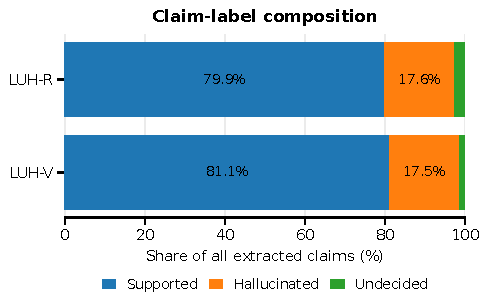
\includegraphics[width=0.98\columnwidth]{figures/fig2_label_distribution.pdf}
\caption{Claim-label composition in the released datasets. Percentages use all extracted claims as the denominator; undecided claims are retained in the datasets but excluded from the supervised binary loss.}
\label{fig:label_distribution}
\end{figure}

\subsection{Split Construction and Overlap Caveat}
\label{sec:split}
The paired data use training, validation, and test partitions of 1,458, 92, and 50 responses, with identical question assignments for both backbones. Questions are selected at even intervals across the ordered entity pool rather than in contiguous blocks, and each selected base entity contributes one question. This does not establish concept-, synonym-, or alias-disjointness, since related entities may have different surface forms. We omit numerical overlap estimates because earlier calculations were not reliable; results are therefore response-level held-out results, not evidence of generalization to strictly unseen concepts.

\subsection{Claim Extraction and Token Alignment}
\label{sec:align}
Responses are segmented at sentence-final punctuation and line breaks; unterminated trailing fragments and sentences shorter than 40 characters after markup removal are discarded. DeepSeek-V4-Flash extracts atomic claims and identifies the words expressing each claim. We match those words greedily and in order to the sentence, create a character mask, and align every overlapping Aya-Expanse token. Claims whose words cannot be aligned are discarded; a second DeepSeek pass assigns supported, hallucinated, or undecided labels, which are copied to aligned tokens.

As Table~\ref{tab:align} shows, the median claim span is 16 tokens and spans are non-contiguous for 64.5\% (LUH-V) and 73.1\% (LUH-R) of claims. About 21\% of covered tokens belong to multiple claims; 4.7\% and 4.6\% receive both supported and hallucinated labels. In conflicts, the later claim overwrites the earlier label; undecided claims do not overwrite labels.

\begin{table}[ht]

\centering

\small

\caption{Claim-to-token alignment statistics of the two datasets.}

\label{tab:align}

\resizebox{\columnwidth}{!}{%

\begin{tabular}{|l|c|c|}

\hline

& \textbf{LUH-V} & \textbf{LUH-R} \\ \hline

Claims per response (median) & 37 & 33 \\ \hline

Claims per source sentence (mean) & 1.98 & 1.88 \\ \hline

Aligned tokens per claim, median (10th--90th pct.) & 16 (9--24) & 16 (9--26) \\ \hline

Claims with non-contiguous aligned tokens & 64.5\% & 73.1\% \\ \hline

Covered tokens shared by $\geq$2 claims & 21.1\% & 21.1\% \\ \hline

Covered tokens with conflicting labels & 4.7\% & 4.6\% \\ \hline

Responses whose last sentence was dropped & 14.4\% & 1.4\% \\ \hline

\end{tabular}}

\end{table}

For feature extraction, stored prompt-response text (including the end-of-sequence token) is re-tokenized rather than reusing generation-time token IDs. The backbone is then evaluated by teacher forcing, so features and labels share the same stored-token positions, although tokenization can differ from the original generation. Span alignment itself has not been separately validated by human annotators, the number of unmatched claims was not recorded, and unterminated final sentences are dropped (14.4\% of LUH-V and 1.4\% of LUH-R responses).

\subsection{Annotation Validation}
\label{sec:annval}
Two medical experts independently reviewed 200 claims (100 per dataset) from 87 answers to 49 questions and could consult medical sources. The sample was quota-sampled (40\% judge-labeled hallucinated, 50\% supported, 10\% undecided); results are reported on the sample and re-weighted to the full-dataset class mix. Experts saw the question, generated answer with source sentence marked, and claim, but not the automatic label or backbone, and selected \emph{correct}, \emph{incorrect}, or \emph{cannot decide}.

Three-way expert agreement was 91.5\% ($\kappa=0.855$), increasing to 95.9\% ($\kappa=0.914$) when undecided labels were excluded. With incorrect as the positive class, the DeepSeek judge achieved $\kappa=0.83$ and 0.73 against the two experts (precision/recall 0.86/0.96 and 0.80/0.88). On 160 claims for which both experts agreed, judge agreement was $\kappa=0.82$, or 0.81 after re-weighting (precision and recall 0.85). Seventeen expert-disagreement cases were excluded from this last comparison. Per-dataset agreement was $\kappa=0.89$ (LUH-V) and 0.75 (LUH-R), based on 77--83 claims each. This review validates a subset of the 114,643 automatically labeled claims, not the entire dataset.

\begin{table}[ht]

\centering

\small

\caption{Agreement between the two medical experts and between the DeepSeek judge and the experts (95\% cluster-bootstrap intervals over answers; incorrect is the positive class; $n$ = claims compared).}

\label{tab:annval}

\resizebox{\columnwidth}{!}{%

\begin{tabular}{|l|c|c|c|c|}

\hline

\textbf{Comparison} & $n$ & \textbf{$\kappa$ [95\% CI]} & \textbf{Prec.} & \textbf{Rec.} \\ \hline

Medical expert 1 vs 2, three labels & 200 & 0.855 [0.79, 0.92] & -- & -- \\ \hline

Medical expert 1 vs 2, correct/incorrect & 170 & 0.914 [0.84, 0.96] & -- & -- \\ \hline

Judge vs medical expert 1 & 171 & 0.83 [0.74, 0.91] & 0.86 & 0.96 \\ \hline

Judge vs medical expert 2 & 171 & 0.73 [0.63, 0.82] & 0.80 & 0.88 \\ \hline

Judge vs claims both experts agree on & 160 & 0.82 [0.73, 0.90] & 0.85 & 0.95 \\ \hline

Same, re-weighted to dataset class mix & 160 & 0.81 [0.70, 0.91] & 0.85 & 0.85 \\ \hline

\end{tabular}}

\end{table}

\section{Uncertainty Head}

\subsection{Architecture}

We train a claim-level head over each frozen backbone. The head pools token-level signals associated with each claim and produces one hallucination score per claim, matching the granularity of the labels and the intended downstream use. We do not fine-tune the underlying language model.
Following the LUH design~\cite{b1}, the head receives two feature families. The first is the backbone's attention history from all layers, using an attention-history size of three preceding positions without pooling at the feature-extraction stage. The second consists of the top-4 token probabilities at each position. These features are concatenated and processed by a two-layer Transformer encoder with hidden dimension 768, eight attention heads, and dropout 0.1. The resulting representation is mapped to a claim-level hallucination prediction.

The backbone parameters remain frozen; only the uncertainty head is trained. The method uses internal signals associated with one generated response and therefore does not require multiple sampled answers or an external retrieval step. In the present implementation, saved responses are re-tokenized and the backbone is evaluated with teacher forcing to recover the feature sequence used by the head (Section~\ref{sec:align}). Thus, ``single-pass'' describes single-response uncertainty estimation in contrast to repeated-generation consistency methods; it should not be read as a claim that the entire pipeline consists of only one forward computation. Feature extraction and auxiliary scoring add computation and memory beyond ordinary text generation.

\subsection{Inference Cost Considerations}

An $N$-sample consistency estimator performs autoregressive decoding for $N$ completions. Our detector instead estimates claim-level risk from internal attention-history and top-4 token-probability signals associated with one response, avoiding the additional $N-1$ generated completions. This is an architectural distinction, not a measured $N$-fold speedup. Feature extraction, attention-tensor retention, token alignment, and the auxiliary Transformer head add computation and may increase peak memory. The memory of repeated sampling also depends on whether completions are processed sequentially or in parallel; sequential sampling need not require $N$ times the peak memory. We did not measure wall-clock latency, feature-extraction time, or peak memory. A matched benchmark is required to establish the net efficiency difference.

\subsection{Training Objective}

For claim $c$, let $y_c=1$ denote a hallucinated claim, $y_c=0$ a supported claim, and $p_c$ the predicted hallucination probability. With $\mathcal{C}$ denoting the labeled claims in a batch, we use weighted binary cross-entropy:

\begin{equation}
\mathcal{L} =
-\frac{1}{|\mathcal{C}|}
\sum_{c\in\mathcal{C}}
\left[
 w_{+} y_c \log p_c + (1-y_c)\log(1-p_c)
\right],
\end{equation}

where $w_{+}$ is 4.64 for Gaokerena-V and 4.53 for Gaokerena-R. The weights compensate for the approximately four-to-one imbalance between supported and hallucinated claims.

Training uses the same optimization configuration for both backbones. The complete configuration is shown in Table~\ref{tab:training}. We do not perform hyperparameter optimization; checkpoint selection is based on validation PR-AUC.

\begin{table}[ht]

\centering

\small

\caption{Training configuration used for both uncertainty heads.}

\label{tab:training}

\resizebox{\columnwidth}{!}{%

\begin{tabular}{|l|c|}

\hline

\textbf{Training setting} & \textbf{Value} \\ \hline

Maximum epochs & 10 \\ \hline

Learning rate & $1\times10^{-4}$ \\ \hline

Warmup ratio & 0.05 \\ \hline

Weight decay & 0.1 \\ \hline

Per-device batch size & 8 \\ \hline

Gradient accumulation & 1 \\ \hline

Maximum gradient norm & 1.0 \\ \hline

Head dimension / layers / heads & 768 / 2 / 8 \\ \hline

Head dropout & 0.1 \\ \hline

Backbone precision & \texttt{fp16} \\ \hline

Checkpoint metric & PR-AUC \\ \hline

Early stopping & 3 epochs \\ \hline

\end{tabular}}

\end{table}

\subsection{Adapter Merging and Reproducibility}

The Gaokerena-V and Gaokerena-R checkpoints are distributed as LoRA adapters rather than standalone language-model weights. The public LUH trainer loads a backbone through a standard model constructor and does not directly handle the Gaokerena PEFT adapter in this path. We therefore load Aya-Expanse-8B, apply each adapter with PEFT, merge the adapter into the base model, and train the uncertainty head against the resulting standalone model. The corresponding Persian claim-level datasets are publicly released as \texttt{gaokerena/LUH\_Gaokerena\_V} (LUH-V) and \texttt{gaokerena/LUH\_Gaokerena\_R} (LUH-R) on Hugging Face. Each release contains 1,600 response records divided into training (1,458), validation (92), and test (50) splits, and exposes the question, response, input token IDs, structured claims, verification labels, and token-level uncertainty labels. The accompanying \texttt{Gaokerena-luh} GitHub repository provides the training and evaluation implementation, trained uncertainty heads, and reproduction documentation.

Both notebooks use half-precision loading for the merged model and the training configuration. Training is performed on a single CUDA GPU with approximately 40~GB of memory at batch size 8. The backbone parameters remain frozen throughout training; only parameters belonging to the uncertainty head are updated.

We also verify tokenizer compatibility before training. The notebooks compare the adapter and base tokenizers and check that chat-template tokenization reproduces the stored input IDs for the test split. This guards against a failure mode in which the supervision refers to token positions generated by a different tokenizer. The stored input IDs are themselves obtained by re-tokenizing the saved response text (see Section~\ref{sec:align}), so this check confirms consistency of the preprocessing rather than equality with generation-time tokenization.

\subsection{Implementation Corrections}

We corrected two issues in the public LUH code. First, recent Transformers versions return a mapping from \texttt{apply\_chat\_template}; treating its length as the token count can shift the reply boundary and place claim masks on prompt tokens. We explicitly extract \texttt{input\_ids} before computing the boundary. Second, the original loader did not reliably resolve the configured PyTorch dtype, so an \texttt{fp16} setting could load the 8B backbone in \texttt{fp32}. We now explicitly map the configuration to the requested torch dtype. These fixes concern preprocessing and loading, not the head architecture.

\subsection{Validation and Test Isolation}

The LUH training framework uses one named validation split internally for evaluation, checkpoint selection, early stopping, and prediction. We therefore configure the 92-response \texttt{eval} split as the validation set during training and do not expose the 50-response \texttt{test} split to checkpoint selection.

After training, a separate evaluation-only run loads the selected head and changes the framework's validation argument to \texttt{test}. The final test metrics therefore do not influence training or model selection. This two-stage procedure avoids using the final test responses as an implicit tuning set. The split construction and the limits of the available overlap analysis are described in Section~\ref{sec:split}; the evaluation is not presented as concept-disjoint.

\section{Results}
\label{sec:results}

Table~\ref{tab:results} reports test performance. Figure~\ref{fig:results} visualizes PR-AUC for our Persian medical models alongside published English-language UHead results. Hallucinated-claim prevalence is 20.95\% for Gaokerena-V (1,951 claims) and 17.46\% for Gaokerena-R (1,687 claims), giving random PR-AUC baselines of 0.2095 and 0.1746. Because an always-negative classifier would achieve 79.05\% and 82.54\% accuracy, accuracy alone is not informative.

\begin{table}[ht]

\centering

\small

\caption{Claim-level uncertainty-head performance on the held-out test splits (\%).}

\label{tab:results}

\resizebox{\columnwidth}{!}{%

\begin{tabular}{|l|c|c|}

\hline

\textbf{Metric} & \textbf{Gaokerena-V} & \textbf{Gaokerena-R} \\ \hline

Accuracy & 76.24 & 62.96 \\ \hline

Precision & 44.85 & 29.52 \\ \hline

Recall & 58.17 & 80.84 \\ \hline

F1 & 50.65 & 43.24 \\ \hline

ROC-AUC & 78.52 & 78.10 \\ \hline

PR-AUC & 48.20 & 46.52 \\ \hline

Random PR-AUC & 20.95 & 17.46 \\
 (base rate) & &  \\ \hline

PR-AUC / random & 2.30 & 2.66 \\ \hline

Test claims & 1,951 & 1,687 \\ \hline

Selected epoch & 3 & 4 \\ \hline

\end{tabular}}

\end{table}


\begin{figure*}[!t]
\centering
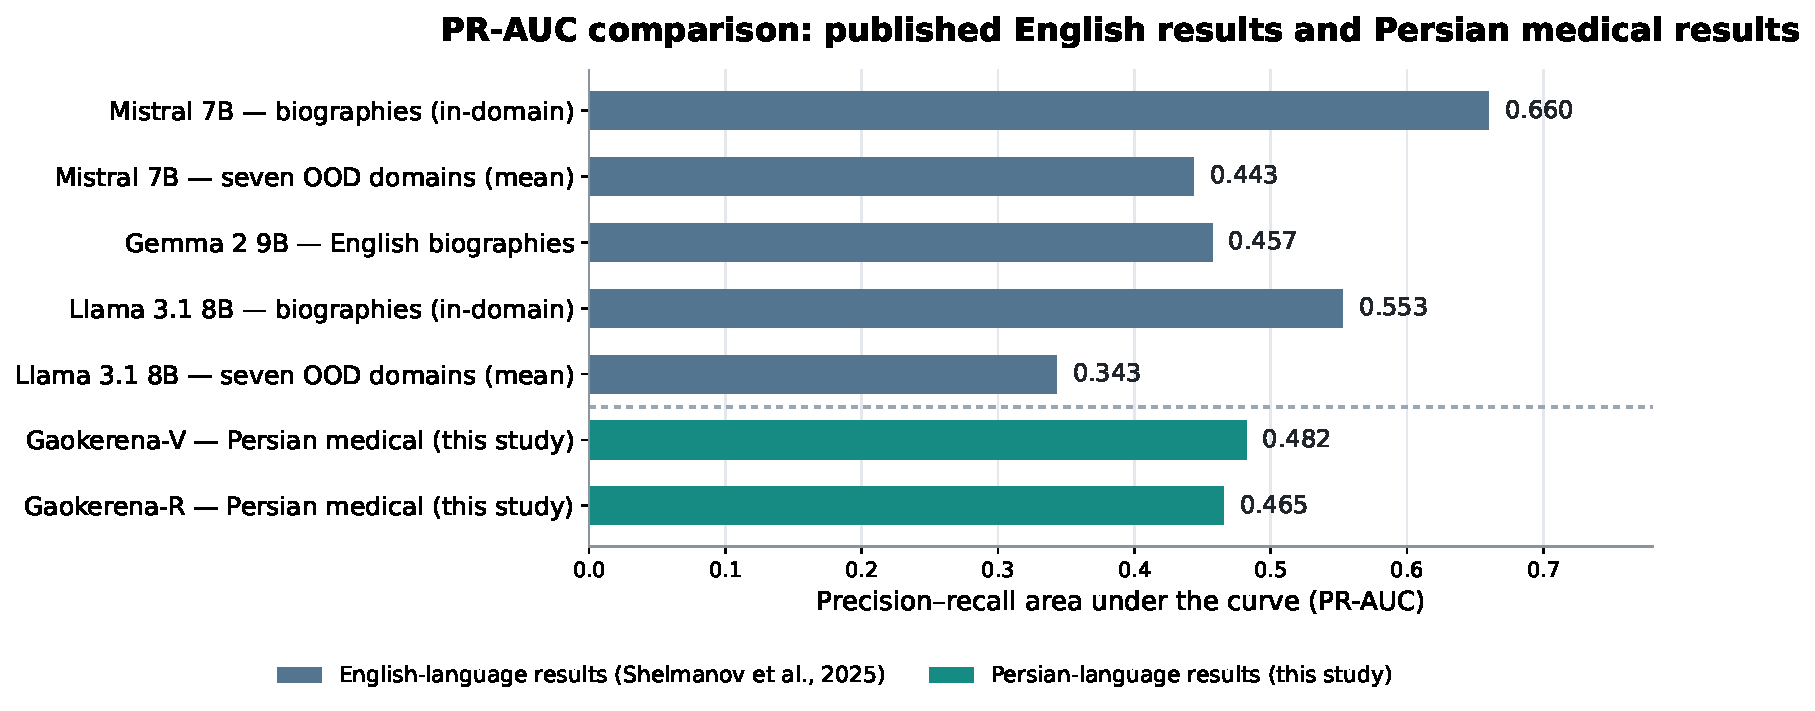
\includegraphics[width=0.96\textwidth]{figures/fig3_pr_auc_comparison.pdf}
\caption{PR-AUC comparison between published English-language results and the Persian medical results in this study. English results are taken from Shelmanov et al.~\cite{b1}: Mistral 7B Instruct v0.2 on English biographies and seven English out-of-domain domains; Gemma 2 9B Instruct on its English biography test set; and Llama 3.1 8B Instruct on English biographies and seven English out-of-domain domains. For the Mistral and Llama out-of-domain groups, the bars show the arithmetic mean across the seven published English domains. No confidence intervals, error bars, or domain-range whiskers are displayed. Gaokerena-V and Gaokerena-R are evaluated on Persian medical data in the present study. This is a contextual cross-study comparison, not a controlled leaderboard, because languages, domains, datasets, annotation procedures, and test distributions differ.}
\label{fig:results}
\end{figure*}

\subsection{Gaokerena-V}

The Gaokerena-V head reaches a PR-AUC of 0.4820 and a ROC-AUC of 0.7852. At the selected operating point, it recalls 58.17\% of hallucinated claims with 44.85\% precision. Its validation PR-AUC reaches 0.4911 at the selected checkpoint, and the final test PR-AUC is 0.4820. The selected checkpoint corresponds to epoch 3, with no later checkpoint improving the validation criterion.

The difference between the random PR-AUC baseline (0.2095) and the observed PR-AUC indicates that the head captures information associated with hallucination labels in the frozen backbone features. This signal is obtained without retrieval, reference passages, or additional generations.

\subsection{Gaokerena-R}

The Gaokerena-R head reaches a PR-AUC of 0.4652 and a ROC-AUC of 0.7810. Its selected operating point has higher recall (80.84\%) and lower precision (29.52\%) than Gaokerena-V. The validation PR-AUC at the selected checkpoint is 0.4108, and the selected checkpoint is epoch 4, followed by early stopping after three epochs without validation improvement.

The lower raw PR-AUC relative to Gaokerena-V should be interpreted alongside the different positive base rates. Relative to the corresponding random floors, the Gaokerena-R and Gaokerena-V heads reach 2.66 and 2.30 times random performance, respectively.

\subsection{Comparison Across Backbones}

The ROC-AUC values are close (0.7852 for Gaokerena-V and 0.7810 for Gaokerena-R), while their precision-recall operating points differ considerably. On these held-out splits, both backbones therefore provide internal signals from which the same LUH-style architecture can learn useful hallucination ranking.

This comparison is enabled by the paired dataset design: both backbones answer the same 1,600 questions, use the same claim-extraction and verification pipeline, and are trained with the same head architecture and optimization settings. The two test splits contain the same 50 questions (Section~\ref{sec:pairing}).

\subsection{Cross-Study PR-AUC Comparison}
The original UHead study reports results for several English-language backbones and domains~\cite{b1}. To make the language distinction explicit, the external results included here are restricted to English evaluations: Mistral 7B Instruct v0.2 obtains a PR-AUC of 0.660 on English biographies (its in-domain test set), while its scores across seven English out-of-domain domains range from 0.340 to 0.561 (mean 0.443). Gemma 2 9B Instruct obtains 0.457 on its English biography test set. Llama 3.1 8B Instruct obtains 0.553 on English biographies and scores from 0.163 to 0.523 across seven English out-of-domain domains (mean 0.343). The means and ranges for the out-of-domain groups are calculated from the seven domain-level values reported in the original paper; they are descriptive summaries, not additional experimental results.

Our Gaokerena-V and Gaokerena-R heads obtain PR-AUCs of 0.4820 and 0.4652, respectively, on Persian medical claim data. Figure~\ref{fig:results} places these Persian results alongside the published English results to provide context for the observed PR-AUC scale. The figure intentionally distinguishes language and evaluation setting: the prior results are English, whereas our results are Persian and medical. It should not be interpreted as a direct model ranking or as evidence that language alone explains performance differences. The underlying backbones, domains, claim datasets, annotation pipelines, positive-class prevalences, and split protocols differ across studies. In addition, the Gemma 2 study reports Russian, Chinese, and German evaluations, but those non-English results are not included in this language-labelled comparison.

The amount of training supervision also differs. The original LUH study reports 3,300 English biography texts for each of its Mistral 7B Instruct v0.2 and Gemma 2 9B Instruct training datasets, containing 68,241 and 83,716 claims, respectively (Table 5 in~\cite{b1}). In our work, each backbone-specific training partition contains 1,458 Persian medical responses, with 55,061 aligned claims for Gaokerena-V and 49,421 for Gaokerena-R. Thus, each of our training partitions contains 55.8\% fewer responses than the original 3,300-text biography datasets.

The smaller size of our training partitions was a consequence of the project budget available for constructing the Persian medical data; it was not selected as a controlled sample-size condition. Despite this constraint, the resulting heads achieve test PR-AUCs of 0.4820 for Gaokerena-V and 0.4652 for Gaokerena-R. These values are 2.30 and 2.66 times the corresponding split-specific random PR-AUC baselines (0.2095 and 0.1746). We regard this as encouraging and acceptable preliminary performance for a budget-constrained adaptation: the internal features provide a useful claim-ranking signal with fewer training responses. This observation should not be interpreted as evidence that our approach is more data-efficient than the original LUH system or that the Persian results are directly comparable to its English results. The language, domain, prompts, claim extraction, annotation, token alignment, and evaluation distributions differ. The claim-count differences are therefore descriptive; our counts include only claims with non-empty token-aligned spans. A controlled learning-curve experiment, varying the number of training responses within the same Persian medical setting, is needed to quantify sample efficiency.

\begin{table}[!b]
\centering
\footnotesize
\setlength{\tabcolsep}{3pt}
\caption{Training-set size and in-domain test PR-AUC in the original LUH study and this work.}
\label{tab:training_scale}
\begin{tabular}{p{0.36\columnwidth}rrp{0.17\columnwidth}}
\toprule
\textbf{Training dataset} & \shortstack{\textbf{Responses/}\\\textbf{texts}} & \textbf{Claims} & \shortstack{\textbf{Test}\\\textbf{PR-AUC}} \\
\midrule
Mistral 7B, English biographies~\cite{b1} & 3,300 & 68,241 & 0.660 \\
Gemma 2 9B, English biographies~\cite{b1} & 3,300 & 83,716 & 0.457 \\
Gaokerena-V, Persian medical (this work) & 1,458 & 55,061 & 0.4820 \\
Gaokerena-R, Persian medical (this work) & 1,458 & 49,421 & 0.4652 \\
\midrule
\multicolumn{4}{p{0.89\columnwidth}}{\footnotesize Note: The original results are for English biography test data; our results are for Persian medical claim data and are not directly comparable. The smaller Persian training partitions reflect the available project budget. Our claim counts include only claims with non-empty token-aligned spans; original LUH counts are reproduced as reported.} \\
\bottomrule
\end{tabular}
\end{table}

The published study also reports that combining attention and token-probability features performed strongly for Mistral 7B on the English biography validation set (PR-AUC 0.642)~\cite{b1}. Our implementation uses the same broad feature families, adapted to the Aya-Expanse-derived Persian backbones. We have not conducted feature-family ablations, so this contextual comparison does not isolate the contribution of attention or probability features in our setting.

\subsection{Review Workload at the Selected Thresholds}

The reported precision, recall, and base rates can be translated into an approximate review workload for the selected checkpoints. On the Gaokerena-V test split, about 530 of 1,951 claims are flagged, corresponding to roughly 27\% of all claims, and about 238 of the flagged claims are hallucinations. On the Gaokerena-R split, about 807 of 1,687 claims are flagged, or roughly 48\% of all claims, again identifying about 238 hallucinated claims. These figures are derived from the reported operating-point metrics and are intended only to illustrate the precision-recall trade-off.

The two workloads illustrate why threshold selection is application-dependent. A reviewer who can inspect only a small fraction of claims would require a stricter operating threshold, while a reviewer prioritizing hallucination recall could accept more false positives. The present experiments use the default threshold of each selected checkpoint rather than tuning the threshold for a specific review budget.

\section{Limitations}
The variability study covers one 168-question examination, five generations per question, and Aya-Expanse-8B plus two evaluated derivatives; it does not characterize every Aya-Expanse model. The dataset uses one question template, lacks medical-specialty labels, and requires fuller documentation of the candidate entity inventory's source and translation. Automatic claim extraction and DeepSeek labels make the resource scalable, while the 200-claim expert review (with access to medical sources) validates only a subset of 114,643 claims. The response-level split is not established as concept- or alias-disjoint; earlier overlap figures are omitted because they were unreliable, and group-disjoint evaluation remains future work. Claim spans are aligned by word matching and character-to-token mapping; stored responses are re-tokenized, and unterminated final sentences are dropped. Finally, we provide no feature-family ablation or measured latency/memory benchmark. The available project budget constrained the size of our Persian training partitions relative to the English biography datasets in the original LUH study. Although our heads achieved PR-AUCs above their respective random baselines, this does not establish sample efficiency: language, domain, prompts, claim extraction, annotation, and evaluation differ across studies, and we did not run a controlled learning-curve experiment. The results therefore support claim ranking above split-specific random PR-AUC baselines, not clinical readiness or a quantified efficiency gain.

\section{Conclusion}
We adapted the LLM Uncertainty Head framework to Persian medical models derived from Aya-Expanse-8B and collected two paired claim-level uncertainty datasets for Persian medical usage. The heads use frozen-backbone attention and token-probability features to estimate hallucination risk for claims in one generated response, without generating multiple completions for consistency comparison. On the held-out response splits, the Gaokerena-V and Gaokerena-R heads achieve ROC-AUCs of 0.7852 and 0.7810 and PR-AUCs of 0.4820 and 0.4652, corresponding to 2.30 and 2.66 times their respective random baselines. The expert review of a 200-claim sample provides an independent check on the automatic labels. Separately, the five-run examination experiment shows that Aya-Expanse-8B and its two evaluated Persian medical derivatives do not have identical response-consistency profiles. This is a caution against assuming that model lineage or medical adaptation guarantees reliability, rather than a claim about every member or derivative of the Aya-Expanse family. The method avoids repeated answer generation but adds feature-extraction and auxiliary-head computation; because end-to-end latency and peak memory were not measured, no quantitative efficiency improvement is claimed. Future work should use verified concept-disjoint evaluation, broader expert annotation, and controlled runtime benchmarks.

\section*{Data and Code Availability}
The paired Persian medical uncertainty datasets are publicly available on Hugging Face Datasets: \texttt{LUH\_Gaokerena\_V} at \url{https://huggingface.co/datasets/gaokerena/LUH_Gaokerena_V} and \texttt{LUH\_Gaokerena\_R} at \url{https://huggingface.co/datasets/gaokerena/LUH_Gaokerena_R}. The training and evaluation code, trained uncertainty-head checkpoints, and reproduction documentation are available in the \texttt{Gaokerena-luh} GitHub repository at \url{https://github.com/Mehrdadghassabi/Gaokerena-luh}.

\begin{thebibliography}{00}

\bibitem{b1}

A. Shelmanov et al., ``A head to predict and a head to question: Pre-trained uncertainty quantification heads for hallucination detection in LLM outputs,'' in \emph{Proceedings of the 2025 Conference on Empirical Methods in Natural Language Processing}, pp. 35712--35731, 2025, doi: 10.18653/v1/2025.emnlp-main.1809.

\bibitem{b2}

M. Ghassabi et al., ``Leveraging online data to enhance medical knowledge in a small Persian language model,'' \emph{arXiv preprint arXiv:2505.16000}, 2025.

\bibitem{b3}

M. Ghassabi et al., ``Enhancing reasoning skills in small Persian medical language models can outperform large-scale data training,'' \emph{arXiv preprint arXiv:2510.20059}, 2025.

\bibitem{b4}

Z. Xia et al., ``A survey of uncertainty estimation methods on large language models,'' \emph{arXiv preprint arXiv:2503.00172}, 2025.

\bibitem{b5}

M. Kirchhof, G. Kasneci, and E. Kasneci, ``Position: Uncertainty quantification needs reassessment for large-language model agents,'' \emph{arXiv preprint arXiv:2505.22655}, 2025.

\bibitem{b6}

A. Shelmanov et al., ``Uncertainty quantification for large language models,'' in \emph{Proceedings of the 63rd Annual Meeting of the Association for Computational Linguistics (Volume 5: Tutorial Abstracts)}, 2025.

\bibitem{b7}

J. Ni et al., ``Reasoning with confidence: Efficient verification of LLM reasoning steps via uncertainty heads,'' \emph{arXiv preprint arXiv:2511.06209}, 2025.

\bibitem{b8}

J. Dang et al., ``RLHF can speak many languages: Unlocking multilingual preference optimization for LLMs,'' \emph{arXiv preprint arXiv:2407.02552}, 2024.

\bibitem{b9}

A. Odumakinde et al., ``Multilingual arbitrage: Optimizing data pools to accelerate multilingual progress,'' \emph{arXiv preprint arXiv:2408.14960}, 2024.

\bibitem{b10}

J. Dang et al., ``Aya Expanse: Combining research breakthroughs for a new multilingual frontier,'' \emph{arXiv preprint arXiv:2412.04261}, 2024.

\bibitem{b11}

A. Sellergren et al., ``MedGemma technical report,'' \emph{arXiv preprint arXiv:2507.05201}, 2025.

\bibitem{b12}

J. Wei et al., ``Chain-of-thought prompting elicits reasoning in large language models,'' in \emph{Advances in Neural Information Processing Systems}, vol. 35, 2022, pp. 24824--24837.

\bibitem{b13}

DeepSeek-AI, ``DeepSeek-V4: Towards highly efficient million-token context intelligence,'' Technical report, 2026.

\end{thebibliography}

\end{document}